\section{Аналитическая часть}

В этом разделе будет приведено описание модели трёхмерного объекта.
Также проводится анализ существующих алгоритмов построения трехмерных изображений и выбираются алгоритмы для решения поставленной задачи.

\subsection{Формализация объектов синтезируемой сцены}

Сцена состоит из определенного набора объектов.
\begin{enumerate}
	\item Стандартный геометрический объект --- представляется в виде полигональной сетки. В число рассматриваемых геометрических объектов входят куб, сфера, цилиндр.
	\item Источник света, который представляет собой материальную точку, испускающую лучи света во все стороны.
	\item Камера характеризуется своим пространственным положением и направлением просмотра.
\end{enumerate}

\subsection{Способы описания трехмерных геометрических моделей на сцене}

В компьютерной графике для описания трехмерных геометрических объектов существуют три типа моделей: каркасная, поверхностная и объёмная \cite{applicationcg}.

\begin{itemize}
	\item \textit{Каркасная модель} --- задается информация о вершинах и рёбрах объектов.
	Это простейший вид моделей, так как задается минимум информации. Однако данный вид представления объектов не всегда корректно
	передает форму объекта.
	\item \textit{Поверхностная модель} часто используется в компьютерной графике, кроме информации о вершинах и ребрах, содержит еще информацию о поверхности.
	Недостатком поверхностной модели является отсутствие информации о том, с какой стороны поверхности находится материал.
	\item \textit{Твердотельная модель} отличается от поверхностной тем, что в данной модели к информации о поверхностях добавляется информация о том, с какой стороны расположен материал. Это достигается путем указания направления внутренней нормали.
\end{itemize}

Для решения поставленной задачи не подойдет каркасная модель, так как такая модель не позволяет получить реалистичное изображение. Твердотельная модель также не подойдет, так как по поставленной задачи нет необходимости знать из какого материала будет выполнен тот или иной объект и с какой стороны расположен материал.
Поэтому выбор остается лишь поверхностной модели.

\subsection{Способы задания поверхностных моделей}

Поверхностная модель задается следующими способами \cite{roders}:
\begin{itemize}
	\item \textit{параметрический способ} --- заключается в том, что для получения поверхности нужно дополнительно вычислять функцию, зависящую от параметра. 
	\item \textit{полигональная сетка} --- характеризуется совокупностью вершин, ребер и граней, определяющих форму объекта в трехмерном пространстве.
\end{itemize}

\subsection{Способ хранения полигональной модели}

Рассмотрим существующие способы хранения информации о полигональной сетке.
\begin{itemize}
	\item \textit{Вершинное представление} --- описывает объект множеством вершин, соединенных с другими вершинами.
	Информация о ребрах и гранях неявно присутствует в представлении из-за чего для восстановления исходного тела необходимо обойти все вершины и составить списки граней.
	\item \textit{Cписок граней} --- представляет объект не только множеством вершин, но граней.
	
\end{itemize}

Стоит отметить, что одним из решающих факторов в выборе способа задания модели в данной работе является скорость выполнения преобразований над объектами сцены.
Поэтому наиболее удобным представлением является модель, заданная полигональной сеткой. 
Такая модель позволит избежать проблем при описании сложных объектов сцены. 
Способом хранения полигональной сетки был выбран список граней, так как это даст явное описание граней. 
Этот способ позволит эффективно преобразовывать модели, так как структура будет включать в себя список вершин.

\subsection{Анализ алгоритмов удаления невидимых линий и поверхностей}

%\subsubsection{Алгоритм Робертса}

%Данный алгоритм работает в объектном пространстве, решая задачу только с выпуклыми телами.

%Алгоритм выполняется в 3 этапа \cite{roders}:
%\begin{enumerate}
%	\item Этап подготовки исходных данных.
%	На данном этапе должна быть задана информация о телах. Для каждого тела сцены должна быть сформирована матрица тела V. Размерность матрицы - 4 * $n$, где $n$ – количество граней тела. Каждый столбец матрицы представляет собой четыре коэффициента уравнения плоскости $ax+by+cz+d=0$, проходящей через очередную грань.
	
%	Таким образом, матрица тела будет представлена в следующем виде:
%	\begin{equation}
%		\label{eq:matr}
%		V = \begin{pmatrix}
%			a_{1} & a_{2} & \ldots & a_{n}\\
%			b_{2} & b_{2} & \ldots & b_{n}\\
%			c_{2} & c_{2} & \ddots & c_{n}\\
%			d_{2} & d_{2} & \ldots & d_{n}
%		\end{pmatrix}
%	\end{equation}
%	Матрица тела должна быть сформирована корректно, то есть любая точка, расположенная внутри тела, должна располагаться по положительную сторону от каждой грани тела. В случае, если для очередной грани условие не выполняется, соответствующий столбец матрицы надо умножить на -1.
	
%	\item Этап удаления рёбер, экранируемых самим телом.
%	На данном этапе рассматривается вектор взгляда E= {0 0-1 0}.
%	Для определения невидимых граней достаточно умножить вектор E на матрицу тела V.
%	Отрицательные компоненты полученного вектора будут соответствовать невидимым граням.
	
%	\item Этап удаления невидимых рёбер, экранируемых другими телами сцены.
%	На данном этапе для определения невидимых точек ребра требуется построить луч, соединяющий точку наблюдения с точкой на ребре. Точка будет невидимой, если луч на своём пути встречает в качестве преграды рассматриваемое тело.
%\end{enumerate}

%\textbf{Приемущества:}
%\begin{itemize}
%	\item алгоритм работает в объектном пространстве;
%	\item высокая точность вычисления.
%\end{itemize}

%\textbf{Недостатки:}
%\begin{itemize}
%	\item рост сложности алгоритма – квадрат числа объектов;
%	\item тела сцены должны быть выпуклыми (усложнение алгоритма, так как нужна будет проверка на выпуклость);
%	\item сложность реализации.
%\end{itemize}

\subsubsection{Алгоритм Варнока}

Алгоритм Варнока работает в пространстве изображений.
В основу алгоритма положен принцип «разделяй и властвуй», состоящий в
разбиении области рисунка на более мелкие подобласти (окна).
Единой версии этого алгоритма не существует.
Но все модификации основываются на рекурсивном разбиении окна изображения.
Для каждого окна определяются многоугольники, которые связаны
с ним, и те, у которых легко определить видимость, изображаются.
Если нет, то разбиение на подокна продолжается до тех пор, пока либо нельзя будет принять однозначное решение, либо размер окна не станет равным одному пикселю.
На каждом этапе разбиения осуществляется определение расположения многоугольников относительно текущего окна.
Насколько быстро будет работать данный алгоритм, зависит от сложности сцены.
Так как было решено использовать полигональную сетку, то это может
затормозить выполнение алгоритма.

\textbf{Приемущества:}
\begin{itemize}
	\item меньшие затраты по времени в случае области, содержащий мало информации.
\end{itemize}

\textbf{Недостатки:}
\begin{itemize}
	\item алгоритм работает рекурсивно;
	\item алгоритм работает только в пространстве изображений;
	\item большие затраты по времени в случае области с высоким информационным содержимым.
\end{itemize}

\subsubsection{Алгоритм, использующий Z-буфер}

Алгоритм Z-буфера работает в пространстве изображения.

Буфер кадра (регенерации) используется для заполнения атрибутов (интенсивности) каждого пикселя в пространстве изображения \cite{roders}.
Для него требуется буфер регенерации, в котором запоминаются значения яркости, а также Z-буфер (буфер глубины), куда можно помещать информацию о координате z для каждого пикселя.
Сначала в Z-буфер заносятся минимально возможные значения z, а буфер регенерации заполняется значениями пикселя, описывающими фон.
Затем каждый многоугольник преобразуется в растровую форму и записывается в буфер регенерации, при этом не производится начального упорядочения.
В процессе работы глубина (значение координаты Z ) каждого нового пикселя, который надо занести в буфер кадра, сравнивается с глубиной того пикселя, который уже занесён в Z-буфер.
Если это сравнение показывает, что новый пиксель расположен ближе к наблюдателю, чем пиксель, уже находящийся в буфере кадра, то новый пиксель заносится в буфер кадра.
Кроме того, производится корректировка Z-буфера: в него заносится глубина нового пикселя.
Если же глубина (значение координаты Z) нового пикселя меньше глубины хранящегося в буфере, то никаких действий производить не надо.

На рисунке~\ref{img:z-buffer} представлен пример работы алгоритма Z-буфера.
\begin{figure}[h]
	\centering
	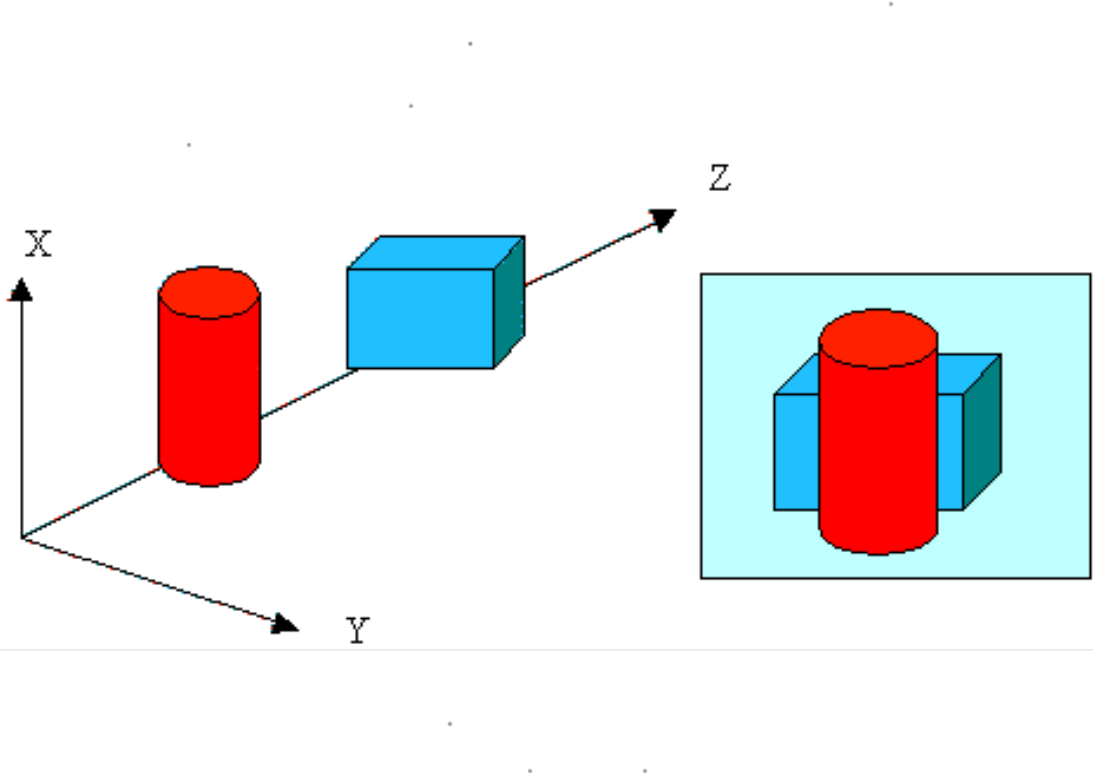
\includegraphics[height=0.35\textheight]{img/z-buffer.png}
	\caption{Алгоритм с Z-буфером \cite{zbuffer}}
	\label{img:z-buffer}
\end{figure}

\textbf{Приемущества:}
\begin{itemize}
	\item простота реализации;
	\item оценка трудоемкости линейна;
	\item отсуствие сортировок.
\end{itemize}

\textbf{Недостатки:}
\begin{itemize}
	\item большой объем требуемой памяти;
	\item эффекты прозначности и просвечивания тяжело реализовать.
\end{itemize}

\subsubsection{Алгоритм обратной трассировки лучей}

Данный алгоритм работает в пространстве изображения.
Основная идея заключается в том, что для каждого пиксела на дисплее проводится прямой луч от наблюдателя до элемента сцены \cite{roders}.
Первое пересечение используется для определения цвета пиксела как функции пересекаемой поверхности элемента.
Также проводятся вторичные лучи от точек пересечения до разных источников света для определения освещённости пиксела.
Если эти лучи блокируются объектом, то данная точка находится в тени, которую отбрасывает рассматриваемый источник света.
Иначе источник света влияет на освещение.
Совокупность всех вторичных лучей, которые достигают источника света, определяет качество освещения, которое попадает на объект сцены.
Также для более реалистичного изображения необходимо проводить лучи отражения и лучи преломления.

\textbf{Приемущества:}
\begin{itemize}
	\item высокая реалистичность синтезируемого изображения;
	\item возможность использования в параллельных вычислительных системах.
\end{itemize}

\textbf{Недостатки:}
\begin{itemize}
	\item производительность.
\end{itemize}
\clearpage
На рисунке~\ref{img:direct-ray-tracing} представлен пример работы алгоритма обратной трассировки лучей.
\begin{figure}[h]
	\centering
	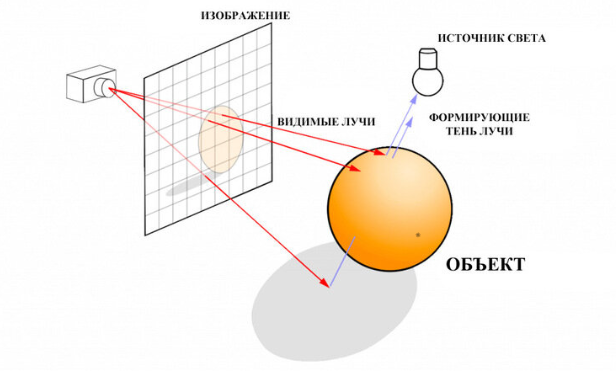
\includegraphics[height=0.3\textheight]{img/direct-ray-tracing.png}
	\caption{Алгоритм обратной трассировки лучей \cite{raytracin}}
	\label{img:direct-ray-tracing}
\end{figure}

\subsubsection{Выбор алгоритма удаления невидимых линий и поверхностей}

При реализации необходимо обеспечить плавную смену кадров при перемещении камеры, поэтому алгоритм должен иметь минимальную зависимость трудоемкости алгоритма от числа объектов на сцене и использование рекурсивных вызовов.

Таким образом, подходящий алгоритм является алгоритм с Z-буфером, который подходит для решения создания сцены с различным количеством объектов, что позволит иметь динамическую сцену.
Данный алгоритм имеет линейную зависимость от числа объектом, что приведет к оптимальной работе программы.
Также он простой в реализации и используется в большинстве графических движков, что приведет к быстрой скорости реализации алгоритма.

\subsection{Анализ алгоритмов закраски}

\subsubsection{Простая закраска}
Один из самых быстрых алгоритмов.
В его основе лежит закон Ламберта, который говорит о том, что интенсивность отражённого света пропорциональна косинусу угла между направлением света и нормалью к поверхности.
Данный метод закраски обладает большим быстродействием, однако все пиксели грани имеют одинаковую интенсивность, и сцена выглядит нереалистично. 
Тем не менее, этот метод крайне прост в реализации и совершенно не требователен к ресурсам.

\subsubsection{Закраска по Гуро}

Метод Гуро устранить дискретность изменения интенсивности и создать иллюзию гладкой криволинейной поверхности.
Он основан на интерполяции интенсивности.

Данный метод отличается от простой закраски тем, что разные точки грани закрашиваются с разными значениями интенсивности.
Для это в каждой вершине грани находится вектор нормали и вычисляется значение интенсивности.
Затем найденные значения интенсивности интерполируются по всем точкам примыкающих граней.

Закрашивание граней по методу Гуро осуществляется в четыре этапа.
\begin{enumerate}
	\item Вычисляются нормали к каждой грани.
	\item Определяются нормали в вершинах. Нормаль в вершине определяется усреднением нормалей примыкающих граней.
	\item На основе нормалей в вершинах вычисляются значения интенсивностей в вершинах согласно выбранной модели отражения света.
	\item Закрашиваются полигоны граней цветом, соответствующим линейной интерполяции значений интенсивности в вершинах.
\end{enumerate}

Метод Гуро применим для небольших граней, расположенных на значительном расстоянии от источника света. Если же размер грани большой, то расстояние от источника света до центра будет меньше, чем до вершин, и центр грани должен выглядеть ярче, чем ребра. 
Но из-за линейного закона, используемого в интерполяции, метод не позволяет это сделать, поэтому появляются участки с неестественной освещенностью

\subsubsection{Закраска по Фонгу}

Закраска Фонга по своей идее похожа на закраску Гуро, но ее отличие состоит в том, что в методе Гуро по всем точкам полигона интерполируется значения интенсивностей, а в методе Фонга – вектора нормалей, и с их помощью для каждой точки находится значение интенсивности~\cite{roders}.

Этапы следующие.
\begin{enumerate}
	\item Определяются нормали к граням.
	\item По нормалям к граням определяются нормали в вершинах. В каждой точке закрашиваемой грани определяется интерполированный вектор нормали.
	\item По направлению векторов нормали определяется цвет точек грани в соответствии с выбранной моделью отражения света.
\end{enumerate}

\subsubsection {Выбор алгоритма закраски}

Алгоритм закраски Фонга требует большего числа вычислений по сравнению с другими.
Так как в данной курсовой работе будут использоваться полигональные сетки и, желательно, чтобы были сглажены границы многоугольников, то лучше всего подойдёт алгоритм закраски по Гуро.

\subsection{Анализ моделей освещения}

Все модели освещения делятся на два вида: глобальные и локальные. 
Глобальные модели учитывают возможности отражения и преломления света от объектов, не являющихся прямыми источниками освещения, поэтому они требуют значительных затрат.

Существуют более простые, локальные модели освещения, которые учитывают только свет от источника. 
Они вычисляют интенсивность, цвет и дальнейшее распределение света на поверхности, но не учитывают перенос света между объектами.  

\subsubsection{Модель Ламберта}
В этой модели воспроизводится идеальное диффузное освещение. Считается, что свет при попадании на поверхность рассеивается равномерно во все стороны.
На рисунке~\ref{img:lambert} показано, что согласно этой модели, освещенность в точке определяется только плотностью света в точке поверхности, а она линейно зависит от косинуса угла падения. 
При этом положение наблюдателя не имеет значения, т.к. диффузно отраженный свет рассеивается равномерно по всем направлениям.

\begin{figure}[h]
	\centering
	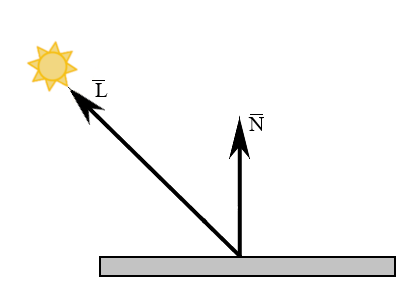
\includegraphics[height=0.3\textheight]{img/lambert.png}
	\caption{Модель освещения Ламберта}
	\label{img:lambert}
\end{figure}

Пусть:
\begin{itemize}
	\item $\overrightarrow L$ --- вектор от точки до источника;
	\item $\overrightarrow N$ --- вектор нормали;
	\item $I$ --- результирующая интенсивность света в точке;
	\item $I_0$ --- интенсивность источника;
	\item $K_d$ --- коэффициент диффузного освещения.
\end{itemize}

Формула расчета интенсивности имеет следующий вид:
\begin{equation}
	\label{eq:lambert}
	I = I_0 \cdot K_d \cdot cos(\overrightarrow L, \overrightarrow N) = I_0 \cdot K_d \cdot (\overrightarrow L, \overrightarrow N) 
\end{equation}
Из формулы (\ref{eq:lambert}) следует главный недостаток модели Ламберта – одинаковая интенсивность во всех точках, принадлежащих одной грани.

Модель Ламберта является одной из самых простых моделей освещения. Данная модель очень часто используется в комбинации других моделей, практически в любой другой модели освещения можно выделить диффузную составляющую.

\subsubsection{Модель Фонга}

Модель Фонга – классическая модель освещения. Модель представляет собой комбинацию диффузной составляющей (модели Ламберта) и зеркальной составляющей и работает таким образом, что кроме равномерного освещения на материале может еще появляться блик.
Падающий и отраженный лучи лежат в одной плоскости с нормалью к отражающей поверхности в точке падения, и эта нормаль делит угол между лучами на две равные части как показано на рисунке~\ref{img:fong-light}.

\begin{figure}[h]
	\centering
	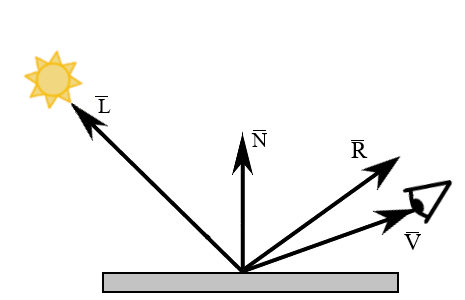
\includegraphics[height=0.3\textheight]{img/phong.png}
	\caption{Модель освещения Фонга}
	\label{img:fong-light}
\end{figure}

Отраженная составляющая освещенности в точке зависит от того, насколько близки направления на наблюдателя и отраженного луча.
Также в модели освещения Фонга используется понятие рассеянного освещения – это константа, которая прибавляется к интенсивности в точке для придания сцене большей реалистичности. 
 
Таким образом, согласно модели Фонга интенсивность к точке складывается будет рассчитываться по формуле: 
\begin{equation}
	\label{eq:simple-model}
	I = I_a + I_d + I_s,
\end{equation}
где $I_a$ --- диффузная составляющая, $I_d$ --- рассеянная  составляющая, $I_s$ --- зеркальная составляющая.
 
\begin{figure}[h]
	\centering
	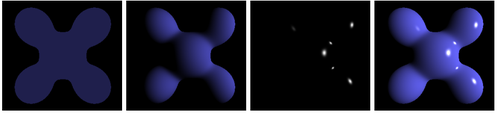
\includegraphics[height=0.15\textheight]{img/phong-model.png}
	\caption{Составляющие модели Фонга (слева направо: рассеянная, диффузная, зеркальная, суммарная)}
	\label{img:fong-model}
\end{figure}

Пусть:
\begin{itemize}
	\item $\overrightarrow R$ --- вектор отраженного луча;
	\item $\overrightarrow V$ --- вектор от точки до наблюдателя;
	\item $I_p$ --- интенсивность рассеянного освещения;
	\item $K_3$ --- коэффициент зеркального освещения;
	\item $K_a$ --- коэффициент рассеянного освещения;
	\item $\alpha$ --- коэффициент блеска.
\end{itemize}
 
Формула для расчета интенсивности для модели Фонга имеет вид:
\begin{equation}
	\label{eq:lambert}
	\begin{aligned}
		I = I_p \cdot K_a  + I_0 \cdot K_d \cdot cos(\overrightarrow L, \overrightarrow N) + I_0 \cdot K_3 \cdot cos^{\alpha}(\overrightarrow R, \overrightarrow V) = \\ = I_p \cdot K_a  + I_0 \cdot K_d \cdot (\overrightarrow L, \overrightarrow N) + I_0 \cdot K_3 \cdot (\overrightarrow R, \overrightarrow V)^{\alpha} 
	\end{aligned}
\end{equation}

\subsubsection{Модель Блинна-Фонга}

Есть большое сходство с моделью Фонга, только она исключает расчёт отражённого луча, что сильно упрощает вычисления, тем самым, экономится время работы.
Но существенной разницы нет.
В этой модели используется медианный вектор, который является единичным и находится посередине между вектором, указывающим направление обзора, и вектором направления освещения.
Чем ближе такой вектор к нормали поверхности, тем больше будет вклад зеркальной компоненты.

Благодаря тому, что измеряется угол между нормалью и медианным вектором (а не между вектором направления наблюдения и вектором отражения, как в модели Фонга), не будет проблемы с резкой границей области зеркального отражения.

\subsubsection{Выбор модели освещения}
В качестве модели освещения была выбрана модель Блинна-Фонга, она позволяет изобразить более реалистичное изображение, чем модель Ламберта, так как учитывает зеркальную составляющую и не требует дополнительных расчётов.
Также такая модель позволяет исключить расчёт отражённого луча, что сильно упрощает вычисления, тем самым, экономится время работы.
\subsection{Перспективно-корректное текстурирование}

Пусть  $u$, $v$ -- координаты текстуры, которые требуется найти для решения задачи наложения текстур на объект трёхмерной сцены.

Метод перспективно-корректного текстурирования основан на приближении $u$ и $v$ кусочно-линейными функциями.
При отрисовке каждая сканирующая строка разбивается на части, в начале и конце каждого куска вычисляются точные значения
$u$ и $v$, а внутри каждой части применяется линейная интерполяция.

Пусть $s_x$ и $s_y$ -- координаты, принадлежащие проекции текстурируемого треугольника.
Тогда значения $ \frac{1}{z} $, $ \frac{u}{z} $ и $ \frac{v}{z} $ линейно зависят от $s_x$ и $s_y$.
Следовательно, для каждой вершины достаточно вычислить значения $ \frac{1}{z} $, $ \frac{u}{z} $ и $ \frac{v}{z} $ и линейно их интерполировать.

Точные значения $ u $ и $ v $ подсчитываются по следующей формуле: 
\begin{equation}
	u = \frac{(u/z)}{1/z},  v = \frac{(u/z)}{1/z} 
\end{equation}

\subsection*{Вывод}
Подведя итог и проанализировав все вышеописанные алгоритмы, можно сделать вывод, что наилучшим алгоритмом для решения задачи будет алгоритм, использующий Z-буфер, модель Фонга-Блинна в сочетании с закраской Гуро. В качестве алгоритма текстиризации был выбран алгоритм перспективно-корректное текстурирование.